\section{Planner  Class Reference}
\label{classPlanner}\index{Planner@{Planner}}
The base class for all path planners. 


{\tt \#include $<$planner.h$>$}

Inheritance diagram for Planner::\begin{figure}[H]
\begin{center}
\leavevmode
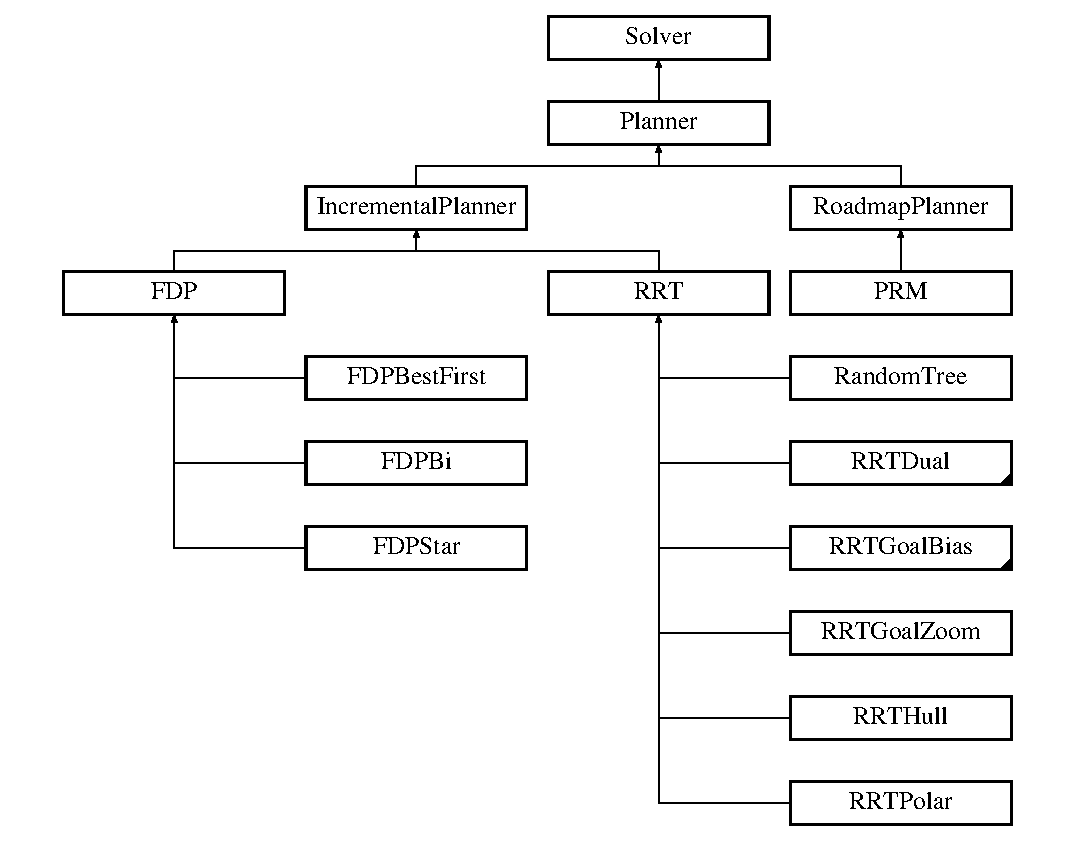
\includegraphics[height=10cm]{classPlanner}
\end{center}
\end{figure}
\subsection*{Public Methods}
\begin{CompactItemize}
\item 
{\bf Planner} ({\bf Problem} $\ast$problem)
\begin{CompactList}\small\item\em A constructor that initializes data members.\item\end{CompactList}\item 
{\bf $\sim$Planner} ()
\item 
void {\bf Reset} ()
\begin{CompactList}\small\item\em Reset the planner.\item\end{CompactList}\item 
virtual void {\bf Construct} ()=0
\begin{CompactList}\small\item\em Generate a planning graph.\item\end{CompactList}\item 
virtual bool {\bf Plan} ()=0
\begin{CompactList}\small\item\em Attempt to solve an Initial-Goal query.\item\end{CompactList}\item 
virtual void {\bf Write\-Graphs} (ofstream \&fout)=0
\begin{CompactList}\small\item\em Write roadmap or trees to a file.\item\end{CompactList}\item 
virtual void {\bf Read\-Graphs} (ifstream \&fin)=0
\begin{CompactList}\small\item\em Read roadmap or trees from a file.\item\end{CompactList}\item 
bool {\bf Gap\-Satisfied} (const {\bf MSLVector} \&x1, const {\bf MSLVector} \&x2)
\begin{CompactList}\small\item\em Determine if the gap error is staisfied.\item\end{CompactList}\end{CompactItemize}
\subsection*{Public Attributes}
\begin{CompactItemize}
\item 
double {\bf Cumulative\-Planning\-Time}
\begin{CompactList}\small\item\em Total amount of time spent on planning.\item\end{CompactList}\item 
double {\bf Cumulative\-Construct\-Time}
\begin{CompactList}\small\item\em Total amount of time spent on construction.\item\end{CompactList}\item 
{\bf list}$<${\bf MSLVector}$>$ {\bf Path}
\begin{CompactList}\small\item\em The solution path, as a {\bf list} {\rm (p.\,\pageref{classlist})} of states.\item\end{CompactList}\item 
{\bf list}$<${\bf MSLVector}$>$ {\bf Policy}
\begin{CompactList}\small\item\em The solution policy, as a {\bf list} {\rm (p.\,\pageref{classlist})} of inputs.\item\end{CompactList}\item 
{\bf MSLVector} {\bf Gap\-State}
\begin{CompactList}\small\item\em The last state in a path before a jump occurs.\item\end{CompactList}\item 
bool {\bf Holonomic}
\begin{CompactList}\small\item\em Set to true to ignore inputs and avoid integration (default false). This will make \char`\"{}regular\char`\"{} path planning much faster.\item\end{CompactList}\item 
{\bf MSLVector} {\bf Gap\-Error}
\begin{CompactList}\small\item\em How much gap error is allowed for each element in bidirectional search.\item\end{CompactList}\item 
{\bf MSLTree}$\ast$ {\bf T}
\begin{CompactList}\small\item\em A search tree (used by incremental planners, but included in Planner base to allow {\bf Gui\-Planner} {\rm (p.\,\pageref{classGuiPlanner})} to handle all planners).\item\end{CompactList}\item 
{\bf MSLTree}$\ast$ {\bf T2}
\begin{CompactList}\small\item\em A second tree (if needed).\item\end{CompactList}\item 
{\bf MSLGraph}$\ast$ {\bf Roadmap}
\begin{CompactList}\small\item\em A graph to represent a roadmap (used by roadmap planners, but included in Planner base to allow {\bf Gui\-Planner} {\rm (p.\,\pageref{classGuiPlanner})} to handle all planners).\item\end{CompactList}\item 
{\bf list}$<$double$>$ {\bf Time\-List}
\begin{CompactList}\small\item\em The times associated with a solution path.\item\end{CompactList}\item 
{\bf list}$<${\bf MSLVector}$>$ {\bf State\-List}
\begin{CompactList}\small\item\em The states associated with a solution path.\item\end{CompactList}\item 
{\bf list}$<${\bf MSLVector}$>$ {\bf Input\-List}
\begin{CompactList}\small\item\em The inputs associated with a solution path.\item\end{CompactList}\item 
int {\bf Num\-Nodes}
\begin{CompactList}\small\item\em Number of nodes to generate in a single execution of Plan or Construct.\item\end{CompactList}\item 
double {\bf Planner\-Delta\-T}
\begin{CompactList}\small\item\em Time step to use for incremental planners.\item\end{CompactList}\end{CompactItemize}
\subsection*{Protected Methods}
\begin{CompactItemize}
\item 
{\bf MSLVector} {\bf Random\-State} ()
\begin{CompactList}\small\item\em Choose a state at random.\item\end{CompactList}\item 
{\bf MSLVector} {\bf Normal\-State} ({\bf MSLVector} mean, double sd)
\begin{CompactList}\small\item\em Pick a state using a Normal distribution.\item\end{CompactList}\end{CompactItemize}
\subsection*{Protected Attributes}
\begin{CompactItemize}
\item 
{\bf MSLRandom\-Source} {\bf R}
\end{CompactItemize}


\subsection{Detailed Description}
The base class for all path planners.



\subsection{Constructor \& Destructor Documentation}
\index{Planner@{Planner}!Planner@{Planner}}
\index{Planner@{Planner}!Planner@{Planner}}
\subsubsection{\setlength{\rightskip}{0pt plus 5cm}Planner::Planner ({\bf Problem} $\ast$ {\em problem})}\label{classPlanner_a0}


A constructor that initializes data members.

\index{Planner@{Planner}!~Planner@{$\sim$Planner}}
\index{~Planner@{$\sim$Planner}!Planner@{Planner}}
\subsubsection{\setlength{\rightskip}{0pt plus 5cm}Planner::$\sim$Planner ()}\label{classPlanner_a1}




\subsection{Member Function Documentation}
\index{Planner@{Planner}!Construct@{Construct}}
\index{Construct@{Construct}!Planner@{Planner}}
\subsubsection{\setlength{\rightskip}{0pt plus 5cm}void Planner::Construct ()\hspace{0.3cm}{\tt  [pure virtual]}}\label{classPlanner_a3}


Generate a planning graph.



Reimplemented in {\bf Incremental\-Planner} {\rm (p.\,\pageref{classIncrementalPlanner_a2})}, and {\bf PRM} {\rm (p.\,\pageref{classPRM_a2})}.\index{Planner@{Planner}!GapSatisfied@{GapSatisfied}}
\index{GapSatisfied@{GapSatisfied}!Planner@{Planner}}
\subsubsection{\setlength{\rightskip}{0pt plus 5cm}bool Planner::Gap\-Satisfied (const {\bf MSLVector} \& {\em x1}, const {\bf MSLVector} \& {\em x2})}\label{classPlanner_a7}


Determine if the gap error is staisfied.

\index{Planner@{Planner}!NormalState@{NormalState}}
\index{NormalState@{NormalState}!Planner@{Planner}}
\subsubsection{\setlength{\rightskip}{0pt plus 5cm}{\bf MSLVector} Planner::Normal\-State ({\bf MSLVector} {\em mean}, double {\em sd} = 0.5)\hspace{0.3cm}{\tt  [protected]}}\label{classPlanner_b1}


Pick a state using a Normal distribution.

\index{Planner@{Planner}!Plan@{Plan}}
\index{Plan@{Plan}!Planner@{Planner}}
\subsubsection{\setlength{\rightskip}{0pt plus 5cm}bool Planner::Plan ()\hspace{0.3cm}{\tt  [pure virtual]}}\label{classPlanner_a4}


Attempt to solve an Initial-Goal query.



Reimplemented in {\bf FDP} {\rm (p.\,\pageref{classFDP_a3})}, {\bf FDPBi} {\rm (p.\,\pageref{classFDPBi_a3})}, {\bf PRM} {\rm (p.\,\pageref{classPRM_a3})}, {\bf RCRRT} {\rm (p.\,\pageref{classRCRRT_a10})}, {\bf RCRRTDual} {\rm (p.\,\pageref{classRCRRTDual_a2})}, {\bf RCRRTExt\-Ext} {\rm (p.\,\pageref{classRCRRTExtExt_a2})}, {\bf RCRRTBall} {\rm (p.\,\pageref{classRCRRTBall_a5})}, {\bf RCRRTBall\-Dual} {\rm (p.\,\pageref{classRCRRTBallDual_a2})}, {\bf RCRRTBall\-Ext\-Ext} {\rm (p.\,\pageref{classRCRRTBallExtExt_a2})}, {\bf RRT} {\rm (p.\,\pageref{classRRT_a3})}, {\bf RRTCon} {\rm (p.\,\pageref{classRRTCon_a2})}, {\bf RRTDual} {\rm (p.\,\pageref{classRRTDual_a2})}, {\bf RRTExt\-Ext} {\rm (p.\,\pageref{classRRTExtExt_a2})}, {\bf RRTExt\-Con} {\rm (p.\,\pageref{classRRTExtCon_a2})}, {\bf RRTCon\-Con} {\rm (p.\,\pageref{classRRTConCon_a2})}, and {\bf RRTBidir\-Balanced} {\rm (p.\,\pageref{classRRTBidirBalanced_a2})}.\index{Planner@{Planner}!RandomState@{RandomState}}
\index{RandomState@{RandomState}!Planner@{Planner}}
\subsubsection{\setlength{\rightskip}{0pt plus 5cm}{\bf MSLVector} Planner::Random\-State ()\hspace{0.3cm}{\tt  [protected]}}\label{classPlanner_b0}


Choose a state at random.

\index{Planner@{Planner}!ReadGraphs@{ReadGraphs}}
\index{ReadGraphs@{ReadGraphs}!Planner@{Planner}}
\subsubsection{\setlength{\rightskip}{0pt plus 5cm}void Planner::Read\-Graphs (ifstream \& {\em fin})\hspace{0.3cm}{\tt  [pure virtual]}}\label{classPlanner_a6}


Read roadmap or trees from a file.



Reimplemented in {\bf Incremental\-Planner} {\rm (p.\,\pageref{classIncrementalPlanner_a6})}, and {\bf Roadmap\-Planner} {\rm (p.\,\pageref{classRoadmapPlanner_a3})}.\index{Planner@{Planner}!Reset@{Reset}}
\index{Reset@{Reset}!Planner@{Planner}}
\subsubsection{\setlength{\rightskip}{0pt plus 5cm}void Planner::Reset ()}\label{classPlanner_a2}


Reset the planner.



Reimplemented in {\bf FDP} {\rm (p.\,\pageref{classFDP_a2})}, {\bf FDPBi} {\rm (p.\,\pageref{classFDPBi_a2})}, and {\bf RRT} {\rm (p.\,\pageref{classRRT_a2})}.\index{Planner@{Planner}!WriteGraphs@{WriteGraphs}}
\index{WriteGraphs@{WriteGraphs}!Planner@{Planner}}
\subsubsection{\setlength{\rightskip}{0pt plus 5cm}void Planner::Write\-Graphs (ofstream \& {\em fout})\hspace{0.3cm}{\tt  [pure virtual]}}\label{classPlanner_a5}


Write roadmap or trees to a file.



Reimplemented in {\bf Incremental\-Planner} {\rm (p.\,\pageref{classIncrementalPlanner_a5})}, and {\bf Roadmap\-Planner} {\rm (p.\,\pageref{classRoadmapPlanner_a2})}.

\subsection{Member Data Documentation}
\index{Planner@{Planner}!CumulativeConstructTime@{CumulativeConstructTime}}
\index{CumulativeConstructTime@{CumulativeConstructTime}!Planner@{Planner}}
\subsubsection{\setlength{\rightskip}{0pt plus 5cm}double Planner::Cumulative\-Construct\-Time}\label{classPlanner_m1}


Total amount of time spent on construction.

\index{Planner@{Planner}!CumulativePlanningTime@{CumulativePlanningTime}}
\index{CumulativePlanningTime@{CumulativePlanningTime}!Planner@{Planner}}
\subsubsection{\setlength{\rightskip}{0pt plus 5cm}double Planner::Cumulative\-Planning\-Time}\label{classPlanner_m0}


Total amount of time spent on planning.

\index{Planner@{Planner}!GapError@{GapError}}
\index{GapError@{GapError}!Planner@{Planner}}
\subsubsection{\setlength{\rightskip}{0pt plus 5cm}{\bf MSLVector} Planner::Gap\-Error}\label{classPlanner_m6}


How much gap error is allowed for each element in bidirectional search.

\index{Planner@{Planner}!GapState@{GapState}}
\index{GapState@{GapState}!Planner@{Planner}}
\subsubsection{\setlength{\rightskip}{0pt plus 5cm}{\bf MSLVector} Planner::Gap\-State}\label{classPlanner_m4}


The last state in a path before a jump occurs.

\index{Planner@{Planner}!Holonomic@{Holonomic}}
\index{Holonomic@{Holonomic}!Planner@{Planner}}
\subsubsection{\setlength{\rightskip}{0pt plus 5cm}bool Planner::Holonomic}\label{classPlanner_m5}


Set to true to ignore inputs and avoid integration (default false). This will make \char`\"{}regular\char`\"{} path planning much faster.

\index{Planner@{Planner}!InputList@{InputList}}
\index{InputList@{InputList}!Planner@{Planner}}
\subsubsection{\setlength{\rightskip}{0pt plus 5cm}{\bf list}$<$ {\bf MSLVector} $>$ Planner::Input\-List}\label{classPlanner_m12}


The inputs associated with a solution path.

\index{Planner@{Planner}!NumNodes@{NumNodes}}
\index{NumNodes@{NumNodes}!Planner@{Planner}}
\subsubsection{\setlength{\rightskip}{0pt plus 5cm}int Planner::Num\-Nodes}\label{classPlanner_m13}


Number of nodes to generate in a single execution of Plan or Construct.

\index{Planner@{Planner}!Path@{Path}}
\index{Path@{Path}!Planner@{Planner}}
\subsubsection{\setlength{\rightskip}{0pt plus 5cm}{\bf list}$<$ {\bf MSLVector} $>$ Planner::Path}\label{classPlanner_m2}


The solution path, as a {\bf list} {\rm (p.\,\pageref{classlist})} of states.

\index{Planner@{Planner}!PlannerDeltaT@{PlannerDeltaT}}
\index{PlannerDeltaT@{PlannerDeltaT}!Planner@{Planner}}
\subsubsection{\setlength{\rightskip}{0pt plus 5cm}double Planner::Planner\-Delta\-T}\label{classPlanner_m14}


Time step to use for incremental planners.

\index{Planner@{Planner}!Policy@{Policy}}
\index{Policy@{Policy}!Planner@{Planner}}
\subsubsection{\setlength{\rightskip}{0pt plus 5cm}{\bf list}$<$ {\bf MSLVector} $>$ Planner::Policy}\label{classPlanner_m3}


The solution policy, as a {\bf list} {\rm (p.\,\pageref{classlist})} of inputs.

\index{Planner@{Planner}!R@{R}}
\index{R@{R}!Planner@{Planner}}
\subsubsection{\setlength{\rightskip}{0pt plus 5cm}{\bf MSLRandom\-Source} Planner::R\hspace{0.3cm}{\tt  [protected]}}\label{classPlanner_n0}


\index{Planner@{Planner}!Roadmap@{Roadmap}}
\index{Roadmap@{Roadmap}!Planner@{Planner}}
\subsubsection{\setlength{\rightskip}{0pt plus 5cm}{\bf MSLGraph} $\ast$ Planner::Roadmap}\label{classPlanner_m9}


A graph to represent a roadmap (used by roadmap planners, but included in Planner base to allow {\bf Gui\-Planner} {\rm (p.\,\pageref{classGuiPlanner})} to handle all planners).

\index{Planner@{Planner}!StateList@{StateList}}
\index{StateList@{StateList}!Planner@{Planner}}
\subsubsection{\setlength{\rightskip}{0pt plus 5cm}{\bf list}$<$ {\bf MSLVector} $>$ Planner::State\-List}\label{classPlanner_m11}


The states associated with a solution path.

\index{Planner@{Planner}!T@{T}}
\index{T@{T}!Planner@{Planner}}
\subsubsection{\setlength{\rightskip}{0pt plus 5cm}{\bf MSLTree} $\ast$ Planner::T}\label{classPlanner_m7}


A search tree (used by incremental planners, but included in Planner base to allow {\bf Gui\-Planner} {\rm (p.\,\pageref{classGuiPlanner})} to handle all planners).

\index{Planner@{Planner}!T2@{T2}}
\index{T2@{T2}!Planner@{Planner}}
\subsubsection{\setlength{\rightskip}{0pt plus 5cm}{\bf MSLTree} $\ast$ Planner::T2}\label{classPlanner_m8}


A second tree (if needed).

\index{Planner@{Planner}!TimeList@{TimeList}}
\index{TimeList@{TimeList}!Planner@{Planner}}
\subsubsection{\setlength{\rightskip}{0pt plus 5cm}{\bf list}$<$ double $>$ Planner::Time\-List}\label{classPlanner_m10}


The times associated with a solution path.



The documentation for this class was generated from the following files:\begin{CompactItemize}
\item 
{\bf planner.h}\item 
{\bf planner.C}\end{CompactItemize}
